\subsection{Maximum Likelihood Estimate}

\begin{definition}[likelihood function]
    If random variables have joint probability $p(x_1,...,x_n\vert \theta)$ then the function $L(\theta\vert x_1,...,x_n)=p(x_1,...,x_n\vert\theta)$ is called the \begriff{likelihood function} of $\theta$.
\end{definition}

The likelihood function tells the probability of getting the data that were observed if the parameter value was really $\theta$.

\begin{definition}[maximum likelihood estimate]
    The \begriff{maximum likelihood estimate} of a parameter $\theta$ is the value that maximizes the likelihood function $L(\theta\vert x_1,...,x_n) = p(x_1,...,x_n\vert\theta)$.
\end{definition}

In practice they maximize the logarithm of the likelihood function and solve the following equation:
\begin{align}
    \frac{\mathrm{d}\log L(\theta\vert x_1,...,x_n)}{\mathrm{d}\theta}\notag
\end{align}

The following formula can find an approximate numerical value for the standard error of almost any maximum likelihood estimator:
\begin{align}
    \SE(\hat{\theta}) \approx\sqrt{-\frac{1}{l''(\hat{\theta})}}\notag
\end{align}
For the 95\% confidence interval we can write:
\begin{align}
    \hat{\theta} - 1.96\cdot\SE(\hat{\theta}) < \theta < \hat{\theta} + 1.96\cdot\SE(\hat{\theta}) \notag
\end{align}
For the 90\% confidence interval we can write:
\begin{align}
    \hat{\theta} - 1.645\cdot\SE(\hat{\theta}) < \theta < \hat{\theta} + 1.645\cdot\SE(\hat{\theta}) \notag
\end{align}

\begin{example}
    The probability density function (PDF) of exponential distribution is
    \begin{align}
        \PDF = \begin{cases}
            \lambda e^{-\lambda x} & x\ge 0 \\ 0 & \text{otherwise}
        \end{cases}\notag
    \end{align}
    We want to estimate the parameter $\lambda$. 
    \begin{center}
       \begin{tabular}{p{4cm}|p{7cm}}
            Likelihood function & $L(\lambda\vert x_1,...,x_n) = \lambda^n e^{-\lambda\sum x_i}$ \\
            \hline
            log-likelihood function & $l(\lambda\vert x_1,...,x_n) = n\log(n)-\lambda\sum x_i$ \\
            \hline
            MLE & $l'(\lambda\vert x_1,...,x_n) = \frac{n}{\lambda} - \sum x_i \overset{!}{=} 0\Rightarrow \hat{\lambda} = \frac{1}{\bar{x}}$ \\
            \hline
            Standard error & $\SE(\hat{\lambda}) = \sqrt{-\frac{1}{l''(\hat{\lambda})}} = \frac{\hat{\lambda}}{\sqrt{n}} = \frac{1}{\sqrt{n}\bar{x}}$ where $l''(\lambda) = -\frac{n}{\lambda^2}$ \\
            \hline
            95\% confidence interval & $\frac{1}{\bar{x}}\pm 1.96\cdot\frac{1}{\sqrt{n}\bar{x}}$
       \end{tabular}
    \end{center}
    
    Lets assume that the mean time between failures of 199 air-conditioners is $\bar{x} = 90.92$ hours. The MLE for the estimated failure rate $\lambda$ is $\frac{1}{\bar{x}} = 0.0110$ failure per hour. \\
    $\Rightarrow$ 95\% confidence interval for the failure rate:
    \begin{align}
        \frac{1}{\bar{x}} \pm 1.96\cdot\frac{1}{\sqrt{n}\bar{x}} \Rightarrow \lambda\in [0.00974,0.01253]\notag
    \end{align}
\end{example}    
    
Given a sample, we can estimate two unknown parameters in a probability distribution, for example, estimate parameters $\mu$ and $\sigma$ in a normal distribution.
    
\begin{definition}[likelihood function for two parameters]
    If random variables have joint probability $p(x_1,...,x_n\vert \theta,\phi)$ then the function $L(\theta,\phi\vert x_1,...,x_n)=p(x_1,...,x_n\vert\theta,\phi)$ is called the \begriff{likelihood function} of $\theta$ and $\phi$.
\end{definition}

The likelihood function is maximised at a turning point of the likelihood function and could therefore be found by setting the partial derivatives of $L(\theta,\phi)$ with respect to $\theta$ and $\phi$ to zero.

There are two important properties of the maximum likelihood estimator $\hat{\theta}$ of a parameter $\theta$ based on a random sample of size $n$ from a distribution with a probability function $p(x_1,...,x_n\vert\theta)$:
\begin{itemize}
    \item Asymptotically unbiased: $E(\hat{\theta})\to\theta$ when $n\to\infty$
    \item Asymptotically has a normal distribution: $\hat{\theta}\to$ normal distribution when $n\to\infty$ that can be used to generate confidence intervals.
    \item Maximum likelihood estimators have low mean squared error if the sample size is large enough. MLE can be heavily biased for small samples!
\end{itemize}

\subsection{Continuous distributions}

The \begriff{lognormal distribution} is used in situations where values are positively skewed, for example, for financial analysis of stock prices. Note that the uncertain variable can increase without limits but cannot take negative values.
\begin{center}
    \begin{tikzpicture}
            \begin{axis}[
		    xmin=0, xmax=2, xlabel=$x$,
		    ymin=0, ymax=1, ylabel=$y$,
		    samples=400,
		    axis y line=middle,
		    axis x line=middle,
		    restrict y to domain=0:1,
		    ]
		    \addplot+[mark=none] {1/(x*sqrt(2*pi))*exp(-0.5*(ln(x))^2)};
		    \addlegendentry{$\mu=0$, $\sigma=1$}
		    \end{axis}
        \end{tikzpicture}
\end{center}

In the \begriff{beta distribution} the uncertain variable is a random value between 0 and  positive value. The distribution is frequently used for estimating the proportions and probabilities (i.e. values between 0 and 1). The shape of the distribution is specified by two positive parameters.

The \begriff{\person{Students} t distribution} is the most widely used distribution in confidence intervals and hypothesis testing. The distribution can be used to estimate the mean of a normally distributed population when the sample size is small. The t distribution comes to approximate the normal distribution as the degrees of freedom (or sample size) increases.
\begin{center}
    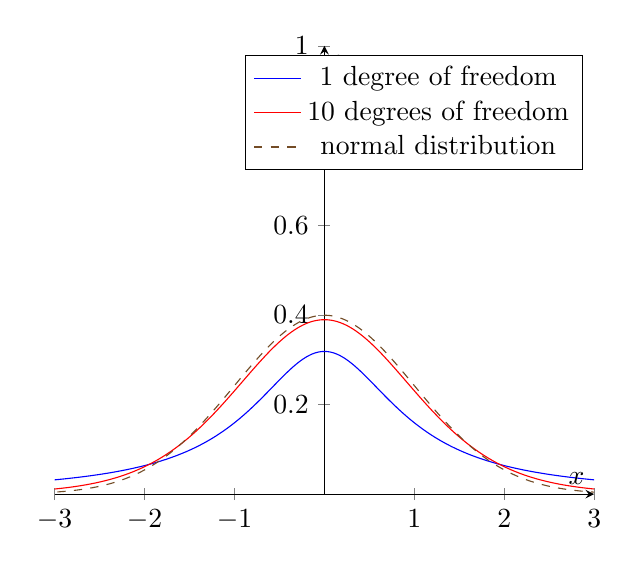
\begin{tikzpicture}
            \begin{axis}[
		    xmin=-3, xmax=3, xlabel=$x$,
		    ymin=0, ymax=1, ylabel=$y$,
		    samples=400,
		    axis y line=middle,
		    axis x line=middle,
		    ]
		    \addplot+[mark=none] {(1)/(pi*(x^2+1))};
		    \addlegendentry{1 degree of freedom}
		    \addplot+[mark=none] {0.389108/((1+x^2/10)^5.5)};
		    \addlegendentry{10 degrees of freedom}
		    \addplot+[dashed,mark=none] {1/(sqrt(2*pi))*exp(-0.5*x^2)};
		    \addlegendentry{normal distribution}
		    \end{axis}
        \end{tikzpicture}
\end{center}

The \begriff{chi-square distribution} is usually used for estimating the variance in a normal distribution.

In a homogeneous \person{Poisson} process with a rate $\lambda$ events per unit time, the time until the first event happens has a distribution called an \begriff{exponential distribution}. All exponential distributions have their highest probability density at $x=0$ and steadily decrease as $x$ increases.
\begin{center}
    \begin{tikzpicture}
            \begin{axis}[
		    xmin=0, xmax=2, xlabel=$x$,
		    ymin=0, ymax=1, ylabel=$y$,
		    samples=400,
		    axis y line=middle,
		    axis x line=middle,
		    restrict y to domain=0:1,
		    ]
		    \addplot+[mark=none] {exp(-x)};
		    \addlegendentry{$\mu=1$}
		    \end{axis}
        \end{tikzpicture}
\end{center}

The \begriff{\person{Weibull} distribution} can be used as a model for items that either deteriorate or improve over time. It's basic version has two parameters: shape and scale.
\begin{center}
    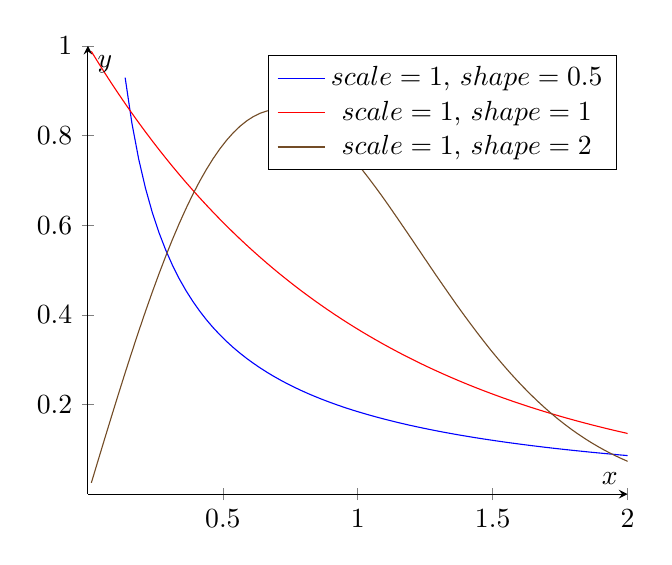
\begin{tikzpicture}
            \begin{axis}[
		    xmin=0, xmax=2, xlabel=$x$,
		    ymin=0, ymax=1, ylabel=$y$,
		    samples=400,
		    axis y line=middle,
		    axis x line=middle,
		    restrict y to domain=0:1,
		    ]
		    \addplot+[mark=none] {0.5*x^(-0.5)*exp(-x^0.5)};
		    \addlegendentry{$scale=1$, $shape=0.5$}
		    \addplot+[mark=none] {1/exp(x)};
		    \addlegendentry{$scale=1$, $shape=1$}
		    \addplot+[mark=none] {2*x^(1)*exp(-x^2)};
		    \addlegendentry{$scale=1$, $shape=2$}
		    \end{axis}
    \end{tikzpicture}
\end{center}
\begin{itemize}
    \item $shape>1$: the hazard function is increasing so the item becomes less reliable as it gets older.
    \item $shape<1$: the hazard function is decreasing so the item becomes more reliable as it gets older.
    \item $shape=1$: the hazard function is constant so the lifetime distribution becomes exponential.
\end{itemize}

The \begriff{survival function} (probability of surviving until a particular time) is $R(t) = 1-F(t)$. The \begriff{hazard rate function} (failure rate) is worked out by the formula:
\begin{align}
    h(t) &= \frac{f(t)}{1-F(t)} \notag \\
    &= \frac{f(t)}{R(t)} \notag
\end{align}
where $f(t)$ and $F(t)$ are PDF and CDF of the distribution.

The hazard function describes how an item ages where $t$ affects its risk of failure. This constant hazard function in the exponential distribution corresponds to the \person{Poisson} process without memory, i.e. the chance of failing does not depend on what happened before and how long the item has already survived.